\documentclass{llncs}
\usepackage{amssymb}
\usepackage{color}
\usepackage{pgf,pgfarrows,pgfnodes,pgfautomata,pgfheaps,pgfshade}
\usepackage{tikz}
\usetikzlibrary{arrows,decorations.pathmorphing,backgrounds,positioning,fit,petri}
\usepackage{amsmath}

\begin{document}

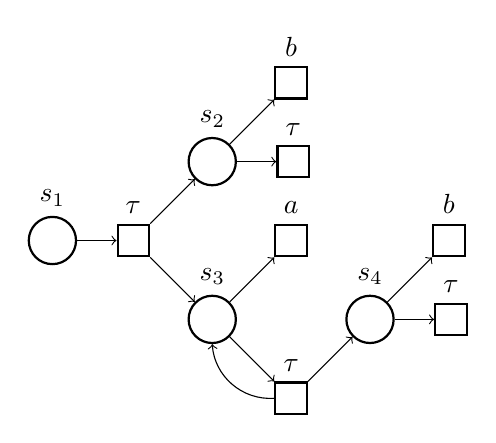
\begin{tikzpicture}[
every place/.style={draw,thick,inner sep=0pt,minimum size=6mm},
every transition/.style={draw,thick,inner sep=0pt,minimum size=4mm},
bend angle=45,
pre/.style={<-,shorten <=1pt,>=stealth,semithick},
post/.style={->,shorten >=1pt,>=stealth,semithick}
]
\def\eofigdist{2.3cm}
\def\eodist{0.5}
\def\eodisty{0.8}


\node (q1) [place] [label={above:$s_1$} ] {};
\node (t1) [transition] [right=\eodist of q1,label=above:$\tau$] {};
\node (q2) [place] [above right=\eodisty of t1,label=above:$s_2$] {};
\node (q3) [place] [below right=\eodisty of t1,label=above:$s_3$] {};
\node (t2) [transition] [right=\eodist of q2,label=above:$\tau$] {};
\node (t21) [transition] [above right=\eodisty of q2,label=above:$b$] {};
\node (t4) [transition] [above right=\eodisty of q3,label=above:$a$] {};
\node (t5) [transition] [below right=\eodisty of q3,label=above:$\tau$] {};
\node (q4) [place] [above right=\eodisty of t5,label=above:$s_4$] {};
\node (t6) [transition] [right=\eodist of q4,label=above:$\tau$] {};
\node (t7) [transition] [above right=\eodisty of q4,label=above:$b$] {};



\draw [->] (q1) to (t1);
\draw [->] (t1) to (q2);
\draw [->] (t1) to (q3);
\draw [->] (q2) to (t2);
\draw [->] (q2) to (t21);
\draw [->] (q3) to (t4);
\draw [->] (q3) to (t5);
\draw [->] (t5) to (q4);
\draw  [->, bend left] (t5) to (q3);
\draw [->] (q4) to (t6);
\draw [->] (q4) to (t7);

\end{tikzpicture}

\end{document}